\documentclass{jsarticle}

 \usepackage{ascmac}
 \usepackage{graphicx}
 \usepackage[dvipdfmx]{color}
 \usepackage{amssymb,amsmath,amsthm}
 \usepackage{graphics}
 \usepackage{fancybox, tcolorbox}
 \tcbuselibrary{raster,skins, breakable}
 \usepackage{nccmath}
 \usepackage{tikz}
 \usetikzlibrary{intersections, calc, cd}
 \usepackage{bm}
 \usepackage[italicdiff]{physics}
 \usepackage{titlesec}
 \usepackage{mathtools}
 \usepackage{enumerate}
 \usepackage{float}

 \numberwithin{equation}{section}
 \setcounter{tocdepth}{3}

\theoremstyle{definition}

\newcommand{\ave}[1]{\langle #1 \rangle}

\usepackage{fancyhdr}
\pagestyle{fancy}
    \lfoot{}
    \cfoot{\thepage}
    \rfoot{}

\begin{document}
キネシンにReduced-VSRを適用するために,つぎのようなモデルを考える.

\begin{figure}[H]
  \begin{center}
  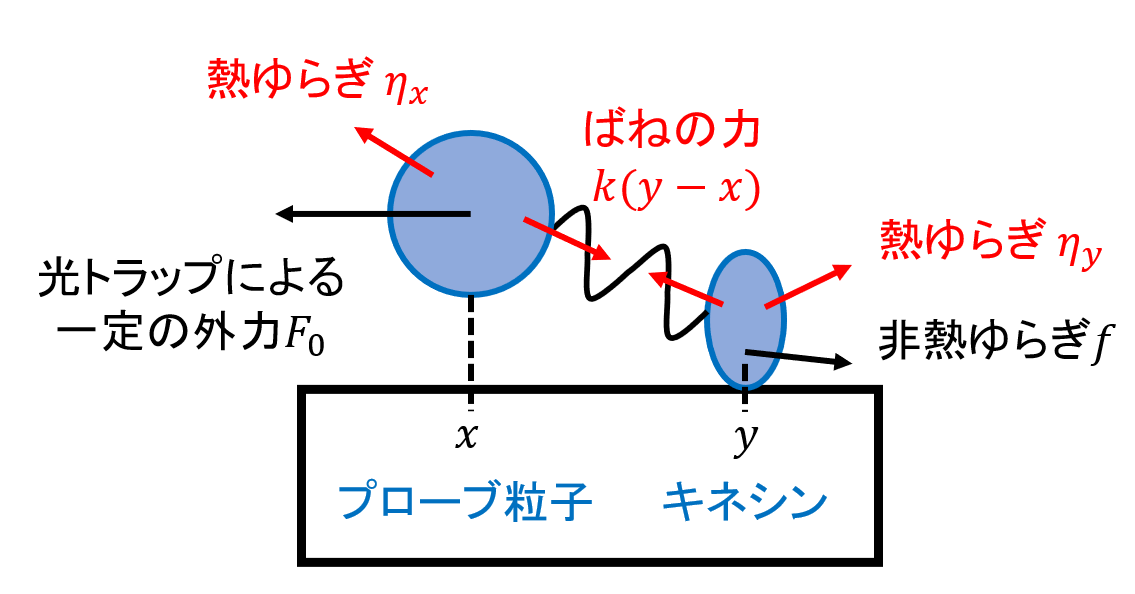
\includegraphics[width=10cm]{kinesine_suggest.png}
  \end{center}
  \caption{提案するキネシンのモデル}
\end{figure}

この場合のオーバーダンプなランジュバン方程式は,つぎの2式.
\begin{equation}
  \dot{x}(t) = \mu_x k (y(t) - x(t)) + F_0 + \sqrt{2D_x} \eta_x (t)
\end{equation}
\begin{equation}
  \dot{y}(t) = - \mu_y k (y(t) - x(t)) + f(t) + \sqrt{2D_y} \eta_y (t)
\end{equation}
いくつかの注意を以下に列挙する.
\begin{itemize}
  \item $x(t)$ はプローブの座標で,$y(t)$ はキネシンの座標である.前者は測定可能だが,後者は測定できない.
  \item $F_0$ は光トラップによる一定の外力
  \item $\ave{\eta_i (t) \eta_j (s)} = \delta_{ij} \delta (t-s)$ であり,熱ゆらぎの大きさは $\sqrt{2D_i}$ に現れる.
  \item $\ave{f(t) f(s)} = \epsilon^2 \exp( - \frac{|t-s|}{\tau_a} )$ を満たすとし,$\tau_a, \epsilon$ はフィッテングにより決定する.
  \item $\mu_i = \gamma_i^{-1}$
  \item $k$ はプローブとキネシンで共通となる.
  \item プローブにかかる非熱ゆらぎ $f$ は,一定の外力 $F_0$ より十分小さいとした.
  \item 光トラップはキネシンには当てないため,$F_0$ が入らない.
\end{itemize}

\end{document}